\section{AFL} \label{sec:2-afl}

Michal Zalewski initially developed American Fuzzy Lopper. He introduces this open-source project as \say{a security-oriented fuzzer that employs a novel type of compile-time instrumentation and genetic algorithms to automatically discover clean, interesting test inputs that trigger new internal states of the targeted binary. This substantially improves the functional coverage for the fuzzed code. The compact synthesized corpora produced by the tool help seed other, more labor- or resource-intensive testing regimes down the road.} \cite{zalewski2014american}

% The algorithm
% Status screen
AFL requires the instrumented binary for execution. To start the instrumentation, AFL uses \textit{afl-clang}, which is built with the coverage recipe included. The following command instruments the sample program \ref{lst:sample_vul}:

\begin{lstlisting}[language=bash,style=CommandStyle,caption=Instrument $sample\_vul$.c]
    afl-clang sample_vul.c -o sample_vul_i
\end{lstlisting}

Now AFL can run this program in \textit{afl-fuzz} with the coverage instrumentations.

\begin{lstlisting}[language=bash,style=CommandStyle,caption=Execute AFL]
  # afl-fuzz -i <in_dir> -o <out_dir> [options] -- /path/to/fuzzed/app [params]
  afl-fuzz -i in_dir -o out_dir -- ./sample_vul_i
\end{lstlisting}

An execution of AFL fuzzing occurs after validating the binary for fuzz testing. The Algorithm \ref{algo:afl} illustrates the execution of \textit{afl-fuzz}:

% main
%     initialize the fuzzer
%     while fuzzing is not terminated:
%         cull the queue of tests and update the bitmap
%         select the first entity of the queue, as E
%         fuzz(E)

% calibrate:
%     /* Calibrate a new test case. This is done when processing the input directory
%    to warn about flaky or otherwise problematic test cases early on; and when
%    new paths are discovered to detect variable behavior and so on. */

% trimming:
%     /* Trim all new test cases to save cycles when doing deterministic checks. The
%    trimmer uses power-of-two increments somewhere between 1/16 and 1/1024 of
%    file size, to keep the stage short and sweet. */

\begin{algorithm}
    % \DontPrintSemicolon % Some LaTeX compilers require you to use \dontprintsemicolon instead
    \KwIn{\textbf{$in\_dir$}, \textbf{$out\_dir$}, $instrumented$ \textbf{$Target$}}
    initialize fuzzer\;
    \While{fuzzing is not terminated} {
      $cull\_queue()$\;
      $Entry \leftarrow q.first\_entry()$\;
      $fuzz\_one(Entry)$\;
    }
    \caption{afl-fuzz}
    \label{algo:afl}
\end{algorithm}

In the fuzzing loop, AFL collects the queue entries and updates the bitmaps for the new entries. Then the first element of the queue is selected for further fuzzing. We demonstrate the pseudocode for fuzzing an entry in Algorithm \ref{algo:fuzzone}:

% fuzz
%     calibrate the test case
%     trim the test cases (if needed)
%     calculate the performance score
%     bitflip
%     interesting values and dictionary usage
%     random havoc

\begin{algorithm}
    \KwIn{\textbf{$queue Entry$}}
    $test\_case \leftarrow Entry.test\_case$
    $calibrate(test\_case)$\;
    $bitflip(test\_case)$\;
    $save\_if\_interesting(test\_case)$\;
    $random\_havoc(test\_case)$\;

    \caption{$fuzz\_one$: Fuzz one Entry}
    \label{algo:fuzzone}
\end{algorithm}

It is noticeable that any newly generated input is executed once before any evaluations.

\subsubsection*{Generate fuzzed data}
AFL generates new inputs after selecting the \textbf{favored inputs}, which are more likely to be selected for more fuzzing.

\begin{itemize}
    \item \textbf{Favored inputs}: After an input is executed, its favor factor is calculated, and later, if it is still interesting for AFL, it is marked as Favored. AFL finds a favorable path for \say{having a minimal set of paths that trigger all the bits seen in the bitmap so far, and focus on fuzzing them at the expense of the rest.} \cite{afl_git} 
    \begin{equation}
        favored\_factor = e.exec\_time \times e.length
        \label{eq:afl_fav_fac}
    \end{equation}
    
    The preference of AFL for the favored inputs increases the performance of AFL in finding new paths. A higher $favored\_factor$ represents a faster execution on smaller inputs.

    \item \textbf{Mutation strategies}: To generate new inputs, AFL takes a queue of inputs and tries mutating and running each one of them. The mutation strategies are in a queue of different strategies that are run on an input to generate more inputs eventually. These strategies include bit-fliping, byte-fliping, simple arithmetic, known integers, stack tweaks, and test case splicing. \cite{afl_strategies}
    
\end{itemize}

\subsubsection*{Status screen}

The \textbf{status screen} is a UI for the status of the fuzzing procedure. As it is shown in Figure \ref{fig:status_screen}, there are multiple stats provided in real-time updates:
    
\begin{figure}[!t]
    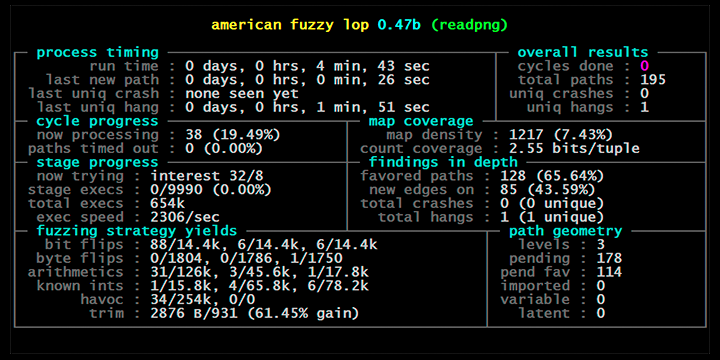
\includegraphics[width=\textwidth]{Chapter2/afl_screen.png}
    \centering
    \caption{AFL status screen}
    \label{fig:status_screen}
\end{figure} 

\begin{enumerate}
    \item \textbf{Process timing}: This section tells about how long the fuzzing process is running.
    \item \textbf{Overall results}: A simplified information about the progress of AFL in finding paths, hangs, and crashes. 
    \item \textbf{Cycle progress}: As mentioned before, AFL takes one input and repeats mutating it for a while. This section shows the information about the current cycle that the fuzzer is working on.
    \item \textbf{Map coverage}: \say{The section provides some trivia about the coverage observed by the instrumentation embedded in the target binary. The first line in the box tells you how many branches we have already hit, in proportion to how much the bitmap can hold. The number on the left describes the current input; the one on the right is the entire input corpus's value. The other line deals with the variability in tuple hit counts seen in the binary. In essence, if every taken branch is always taken a fixed number of times for all the inputs we have tried, this will read "1.00". As we manage to trigger other hit counts for every branch, the needle will start to move toward "8.00" (every bit in the 8-bit map hit) but will probably never reach that extreme. 
    
    Together, the values can help compare the coverage of several different fuzzing jobs that rely on the same instrumented binary.
    }
    \item \textbf{Stage progress}: The information about the current mutation stage is briefly provided here.
    \item \textbf{Findings in depth}: The crashes and hangs and any other findings (here we have the other information about the coverage) are presented in this section.
    \item \textbf{Fuzzing strategy yields}: To illustrate more stats about the strategies used since the beginning of fuzzing, and for comparison of those strategies, AFL keeps track of how many paths were explored, in proportion to the number of executions attempted, for each of the fuzzing strategies.
    \item \textbf{Path geometry}: The information about the inputs and their depths, which says how many generations of different paths were produced in the process. For instance, we call the seeds we provided for fuzzing the "level 1" inputs. Next, a new set of inputs is generated as "level 2", the inputs derived from "level 2" are "level 3," and so on.
\end{enumerate}